\chapter{Appendix: Results}
In this appendix are collected all results of
\begin{itemize}
    \item feature selection evaluated by fs\_results.ipynb;
    \item model prediction errors by Keras\_prediction\_model.ipynb and RandomForest\_prediction\_model.ipynb;
\end{itemize}
\pagebreak
\clearpage
\section{Feature Selection results}
\subsection{Borda Count results}
\begin{figure}[H]
\vspace*{\fill}
\vspace{-\topskip}
\centering
\subfloat[10 Km resolution with mountains]{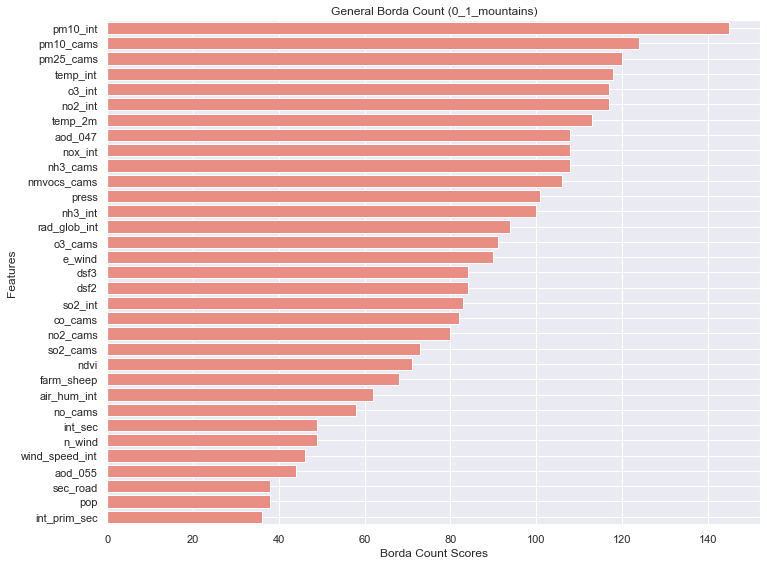
\includegraphics[scale =0.42]{images/tests/0_1_mountainspm25_st.png}}\\
\subfloat[10 Km resolution with mountains]{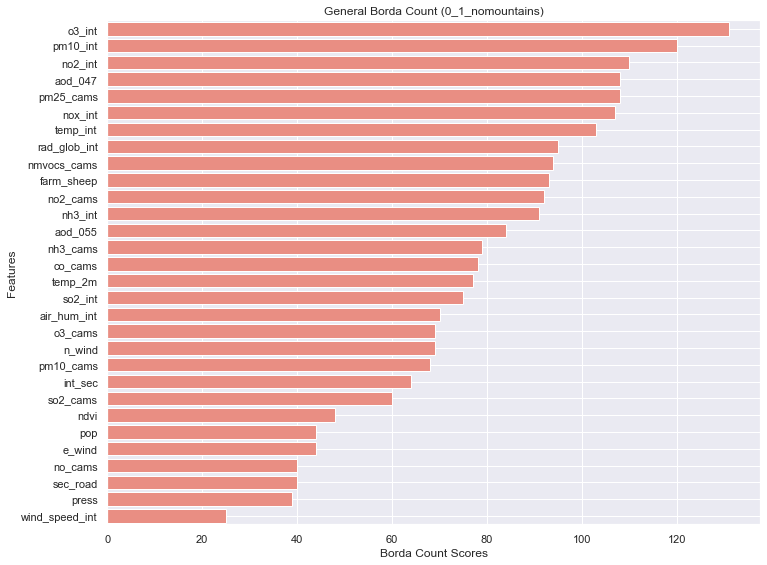
\includegraphics[scale =0.42]{images/tests/0_1_nomountainspm25_st.png}}
\caption{FS results obtained with fine particulate ('pm25\_st') as target variable and 10 km resolution.}
\vspace{\fill}

\end{figure}
\begin{figure}[H]
\centering
\subfloat[10 Km resolution with mountains]{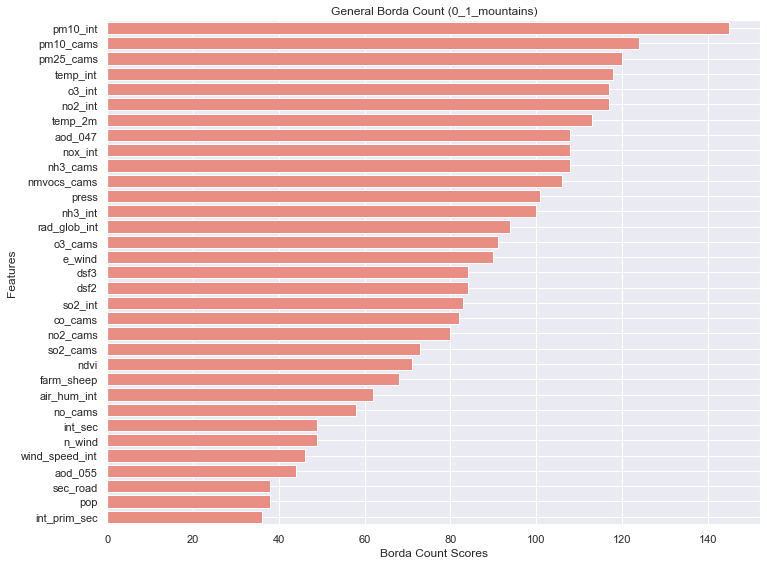
\includegraphics[scale =0.42]{images/tests/0_1_mountainspm25_st.png}}\\
\subfloat[10 Km resolution with mountains]{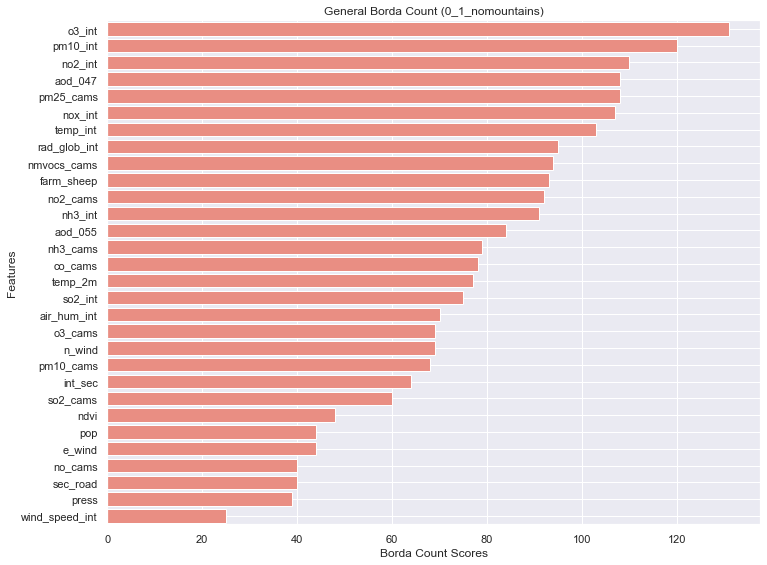
\includegraphics[scale =0.42]{images/tests/0_1_nomountainspm25_st.png}}
\caption{FS results obtained with fine particulate ('pm25\_st') as target variable and 10 km resolution.}
\end{figure}
\begin{figure}[H]
\centering
\subfloat[1 Km resolution with mountains]{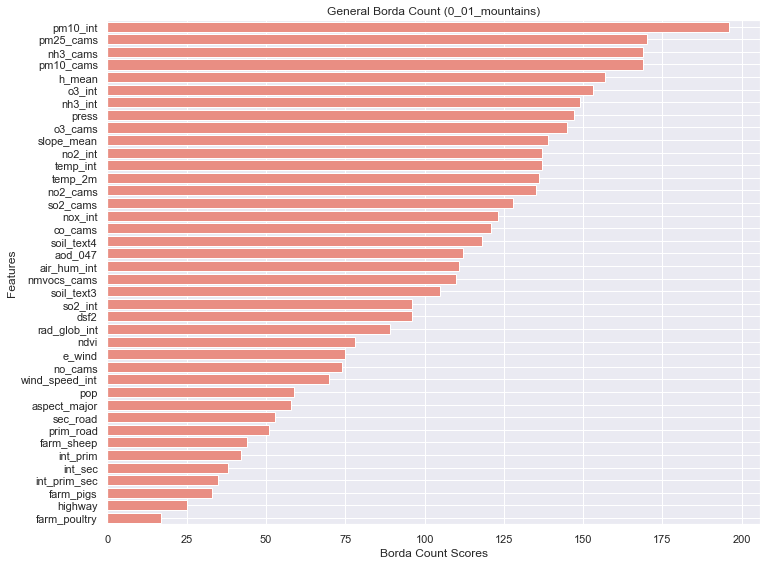
\includegraphics[scale =0.42]{images/tests/0_01_mountainspm25_st.png}}\\
\subfloat[1 Km resolution with mountains]{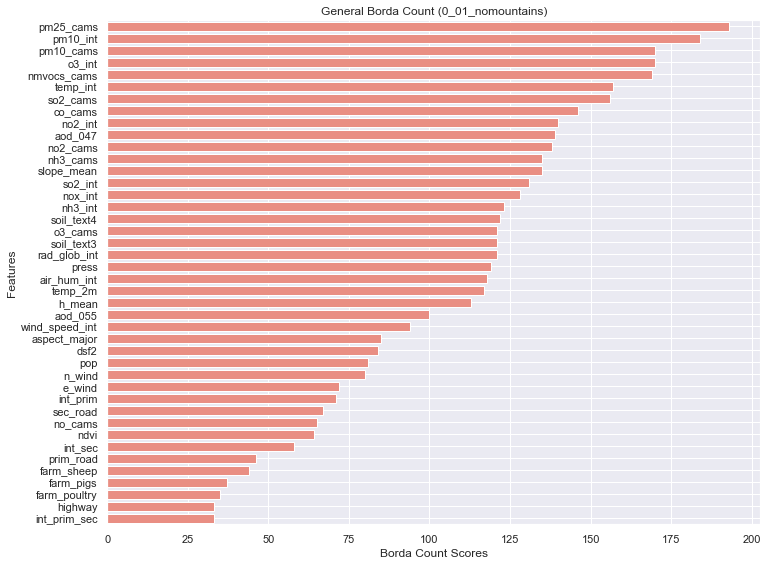
\includegraphics[scale =0.42]{images/tests/0_01_nomountainspm25_st.png}}
\caption{FS results obtained with fine particulate ('pm25\_st') as target variable and 1 km resolution.}
\end{figure}
\begin{figure}[H]
\centering
\subfloat[10 Km resolution with mountains]{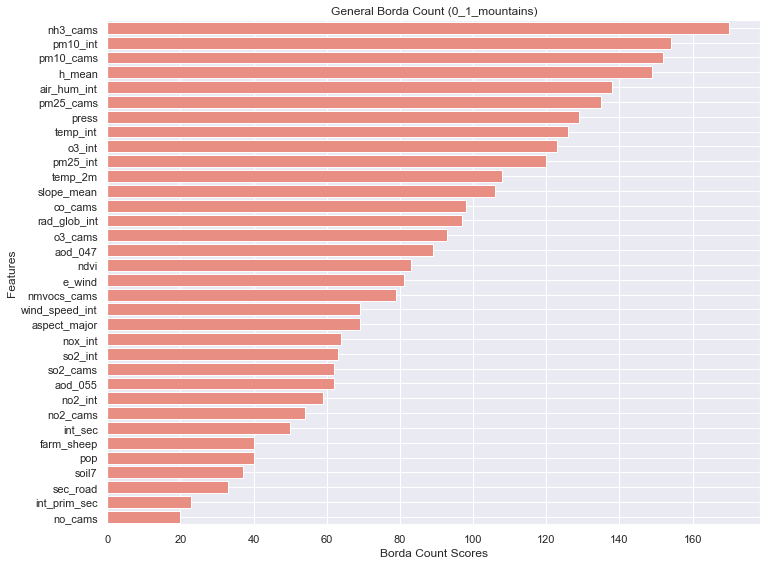
\includegraphics[scale =0.42]{images/tests/0_1_mountainsnh3_st.png}}\\
\subfloat[10 Km resolution with mountains]{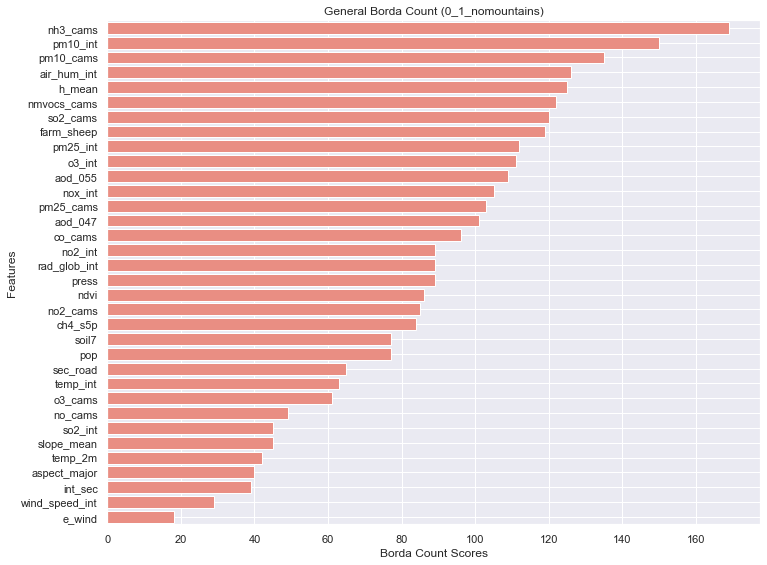
\includegraphics[scale =0.42]{images/tests/0_1_nomountainsnh3_st.png}}
\caption{FS results obtained with ammonia ('nh3\_st') as target variable and 10 km resolution.}
\end{figure}
\begin{figure}[H]
\centering
\subfloat[1 Km resolution with mountains]{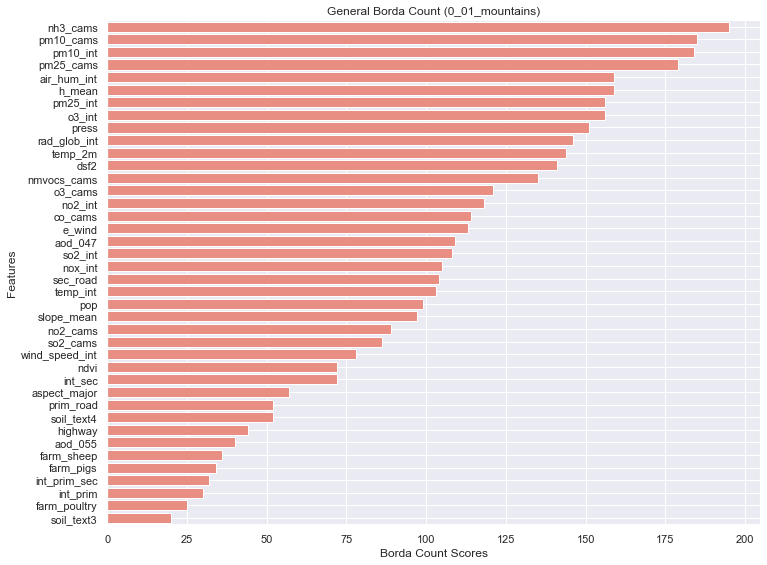
\includegraphics[scale =0.42]{images/tests/0_01_mountainsnh3_st.png}}\\
\subfloat[1 Km resolution with mountains]{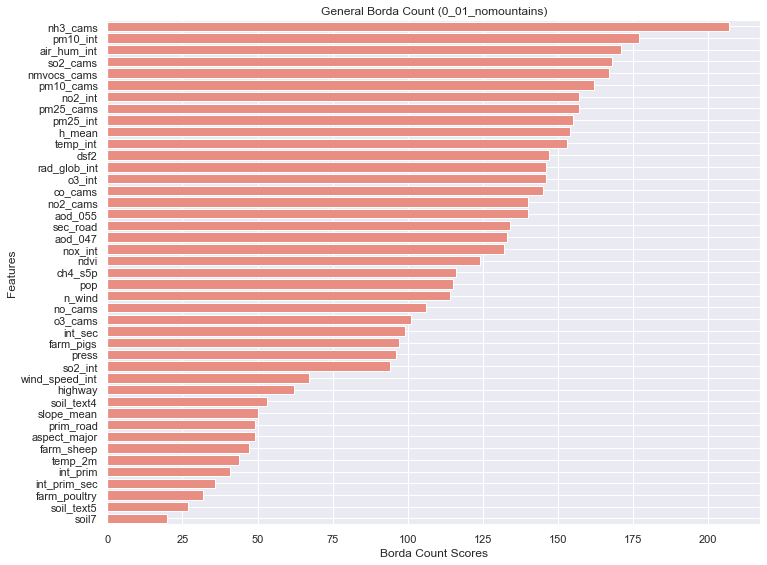
\includegraphics[scale =0.42]{images/tests/0_01_nomountainsnh3_st.png}}
\caption{FS results obtained with ammonia ('nh3\_st') as target variable and 1 km resolution.}
\end{figure}
\subsection{Pearson correlation index results}
\begin{figure}[H]
    \centering
    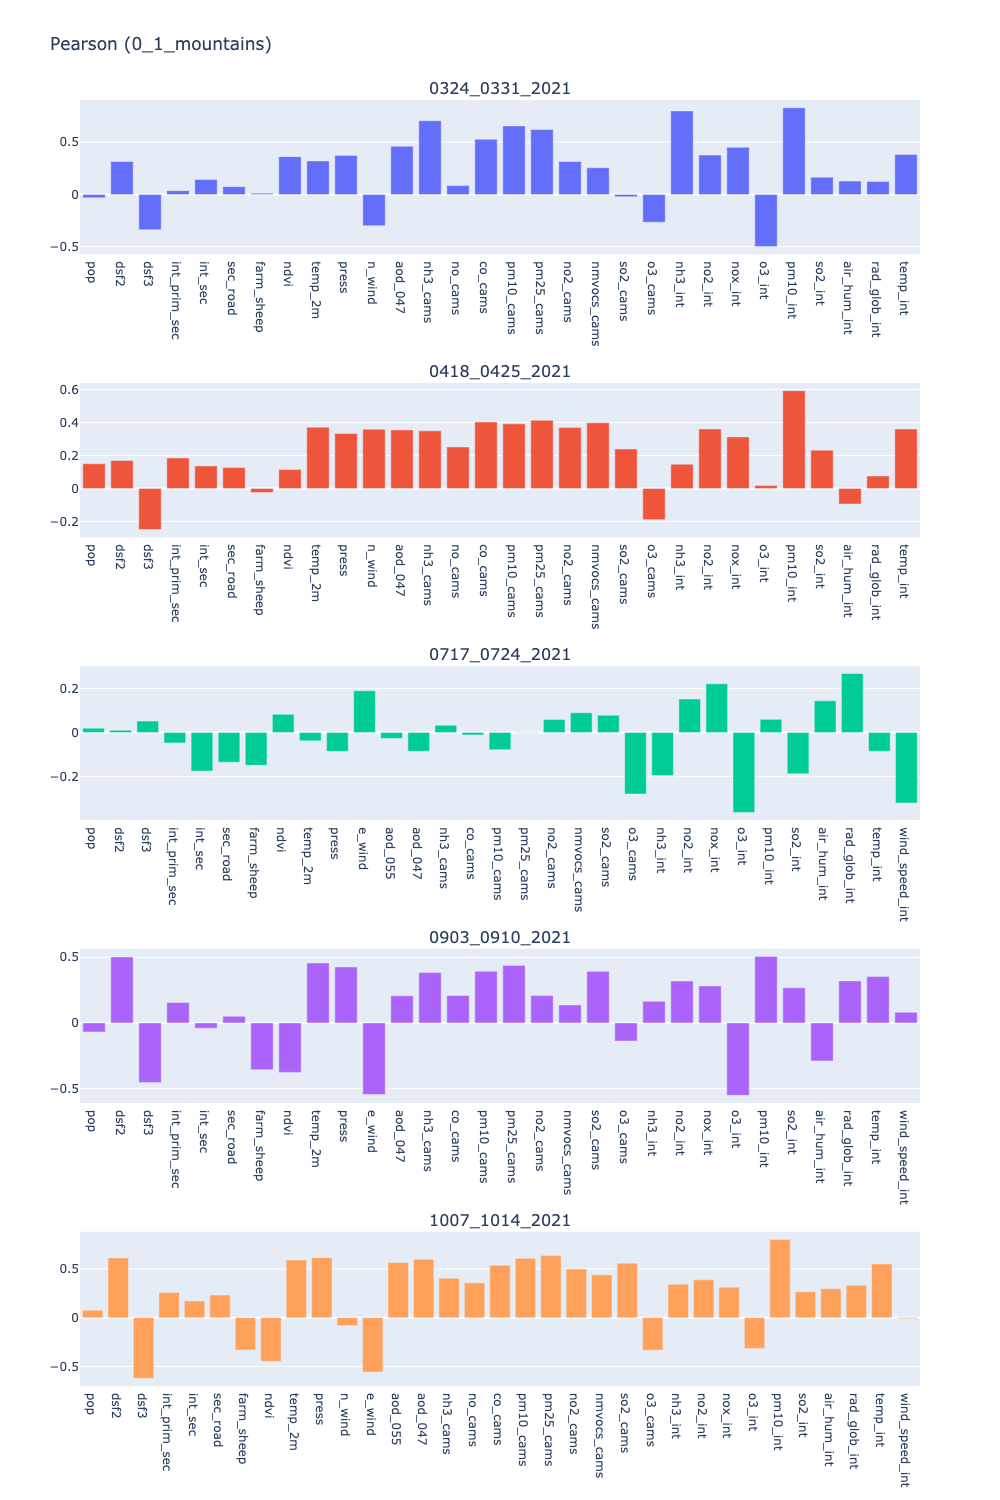
\includegraphics[scale=0.35]{images/tests/0_1_mountainspm25_st_pearson.png}
    \caption{Pearson correlation index results with respect to fine particulate ('pm25\_st') as target variable, with 10km resolution including mountains.}
    \label{fig:overview}
\end{figure}
\begin{figure}[H]
    \centering
    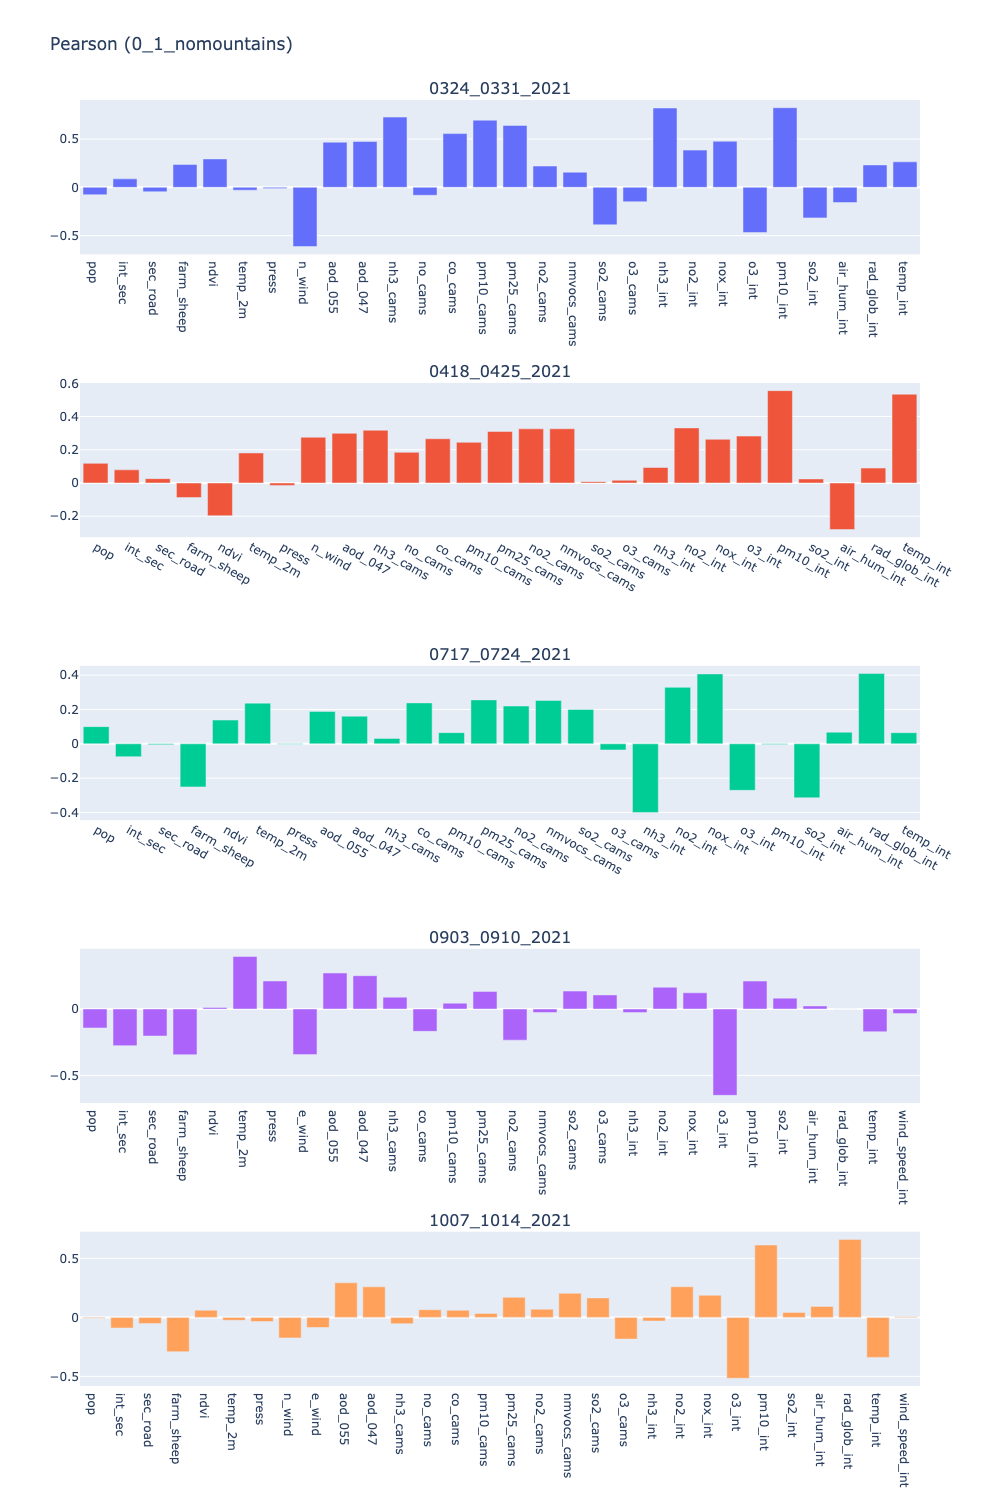
\includegraphics[scale=0.35]{images/tests/0_1_nomountainspm25_st_pearson.png}
    \caption{Pearson correlation index results with respect to fine particulate ('pm25\_st') as target variable, with 10km resolution excluding mountains.}
    \label{fig:overview}
\end{figure}
\begin{figure}[H]
    \centering
    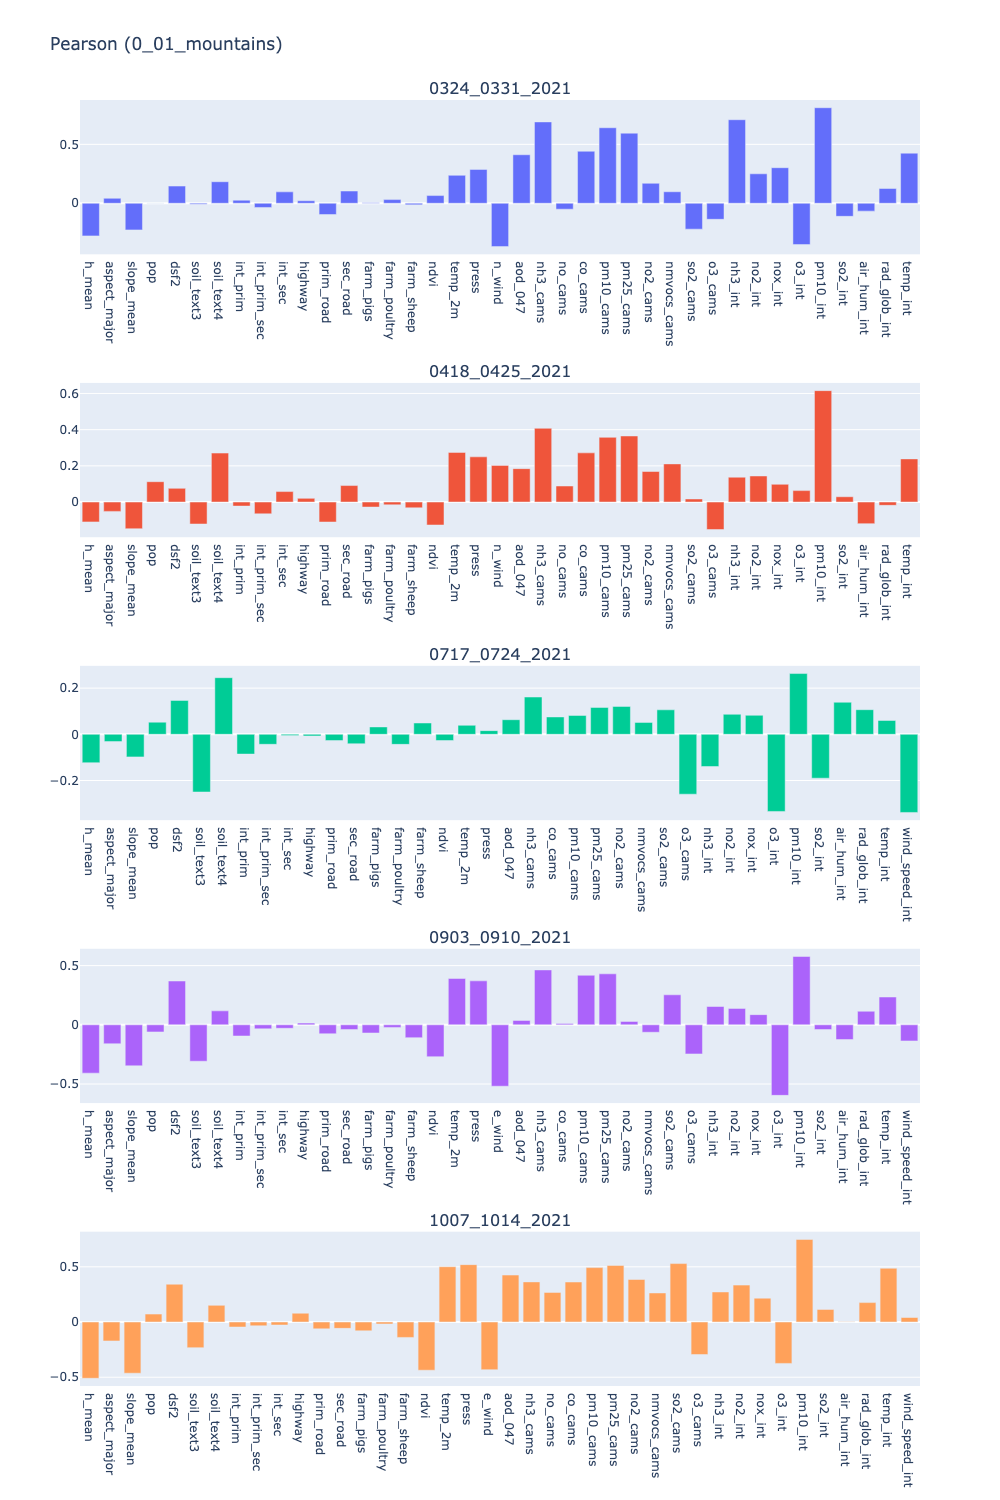
\includegraphics[scale=0.35]{images/tests/0_01_mountainspm25_st_pearson.png}
    \caption{Pearson correlation index results with respect to fine particulate ('pm25\_st') as target variable, with 1km resolution including mountains.}
    \label{fig:overview}
\end{figure}
\begin{figure}[H]
    \centering
    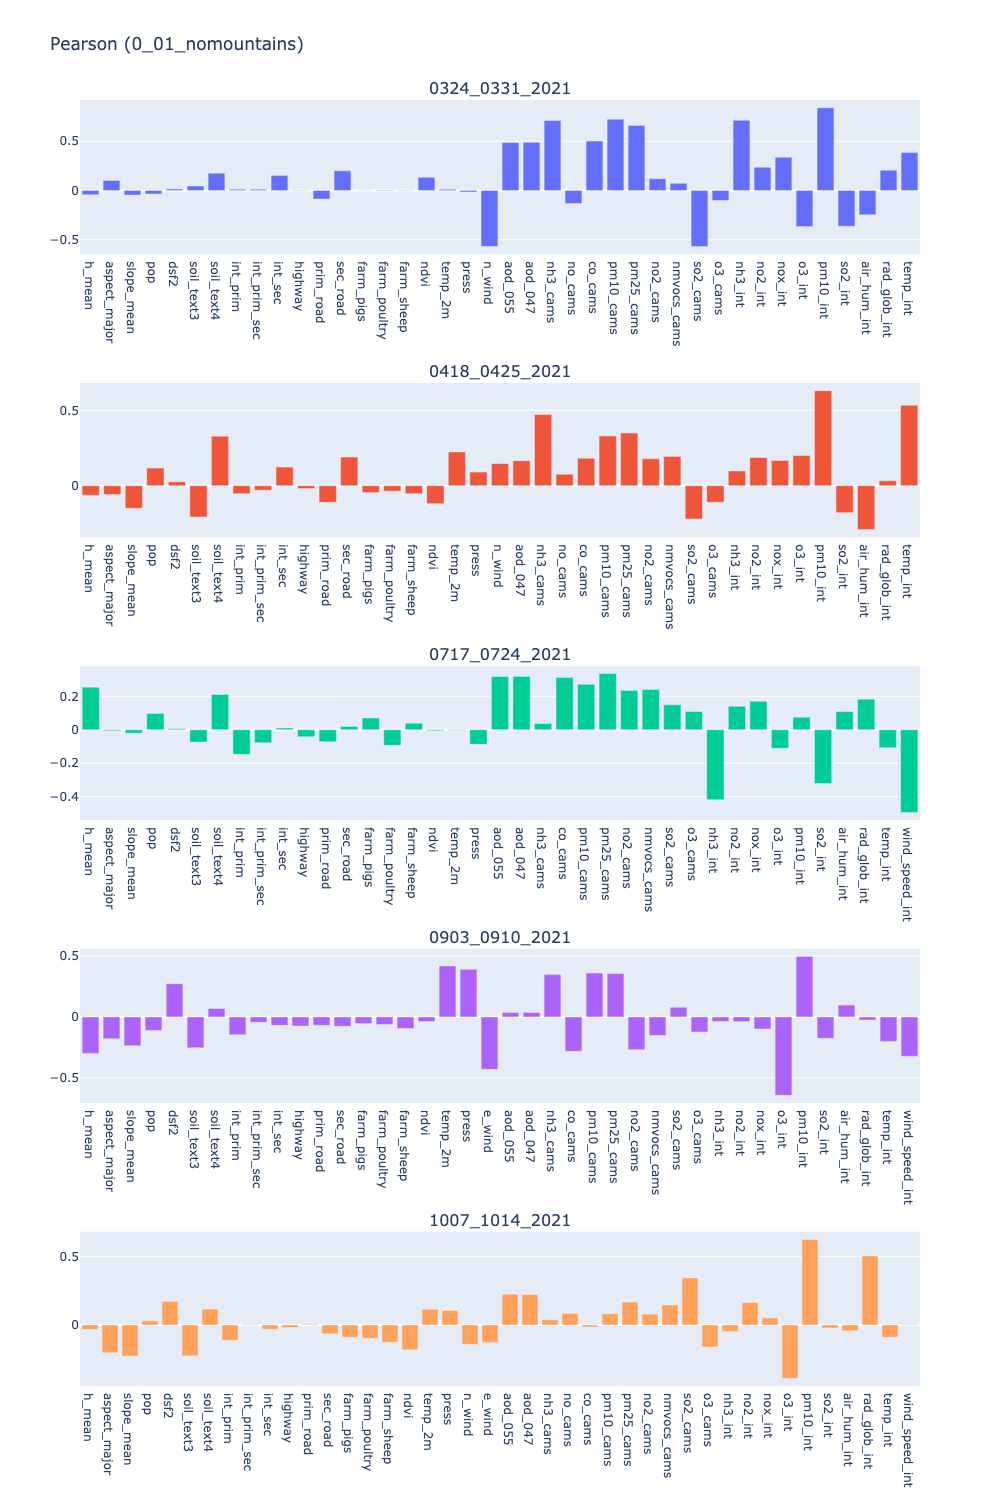
\includegraphics[scale=0.35]{images/tests/0_01_nomountainspm25_st_pearson.png}
    \caption{Pearson correlation index results with respect to fine particulate ('pm25\_st') as target variable, with 1km resolution excluding mountains.}
    \label{fig:overview}
\end{figure}


\begin{figure}[H]
    \centering
    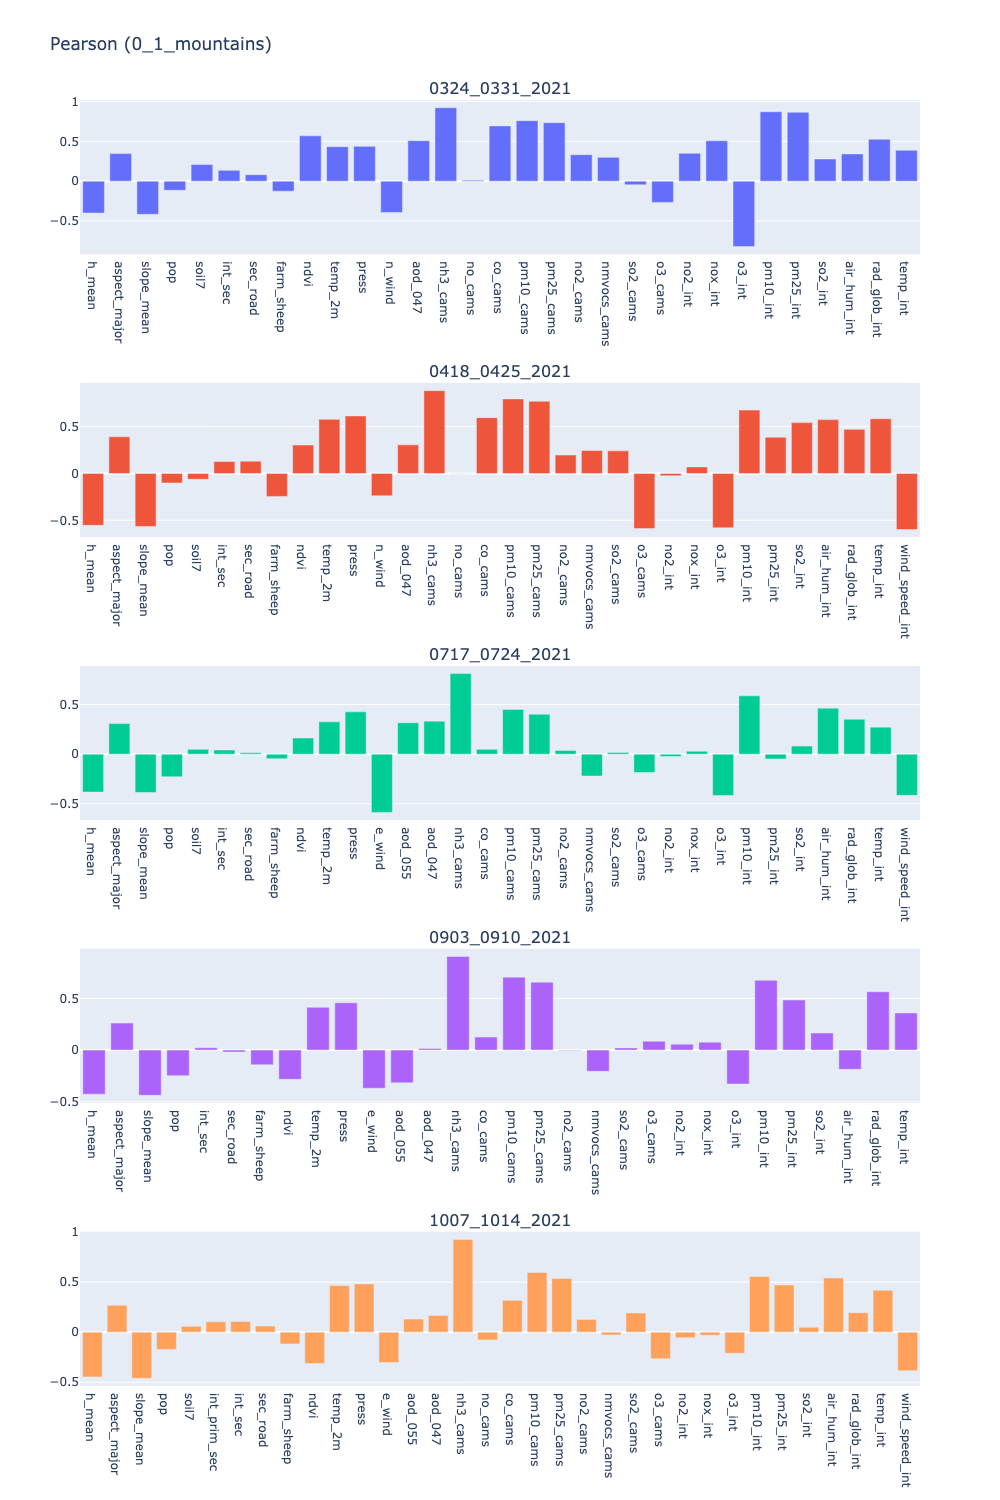
\includegraphics[scale=0.35]{images/tests/0_1_mountainsnh3_st_pearson.png}
    \caption{Pearson correlation index results with respect to ammonia ('nh3\_st') as target variable, with 10km resolution including mountains.}
    \label{fig:overview}
\end{figure}
\begin{figure}[H]
    \centering
    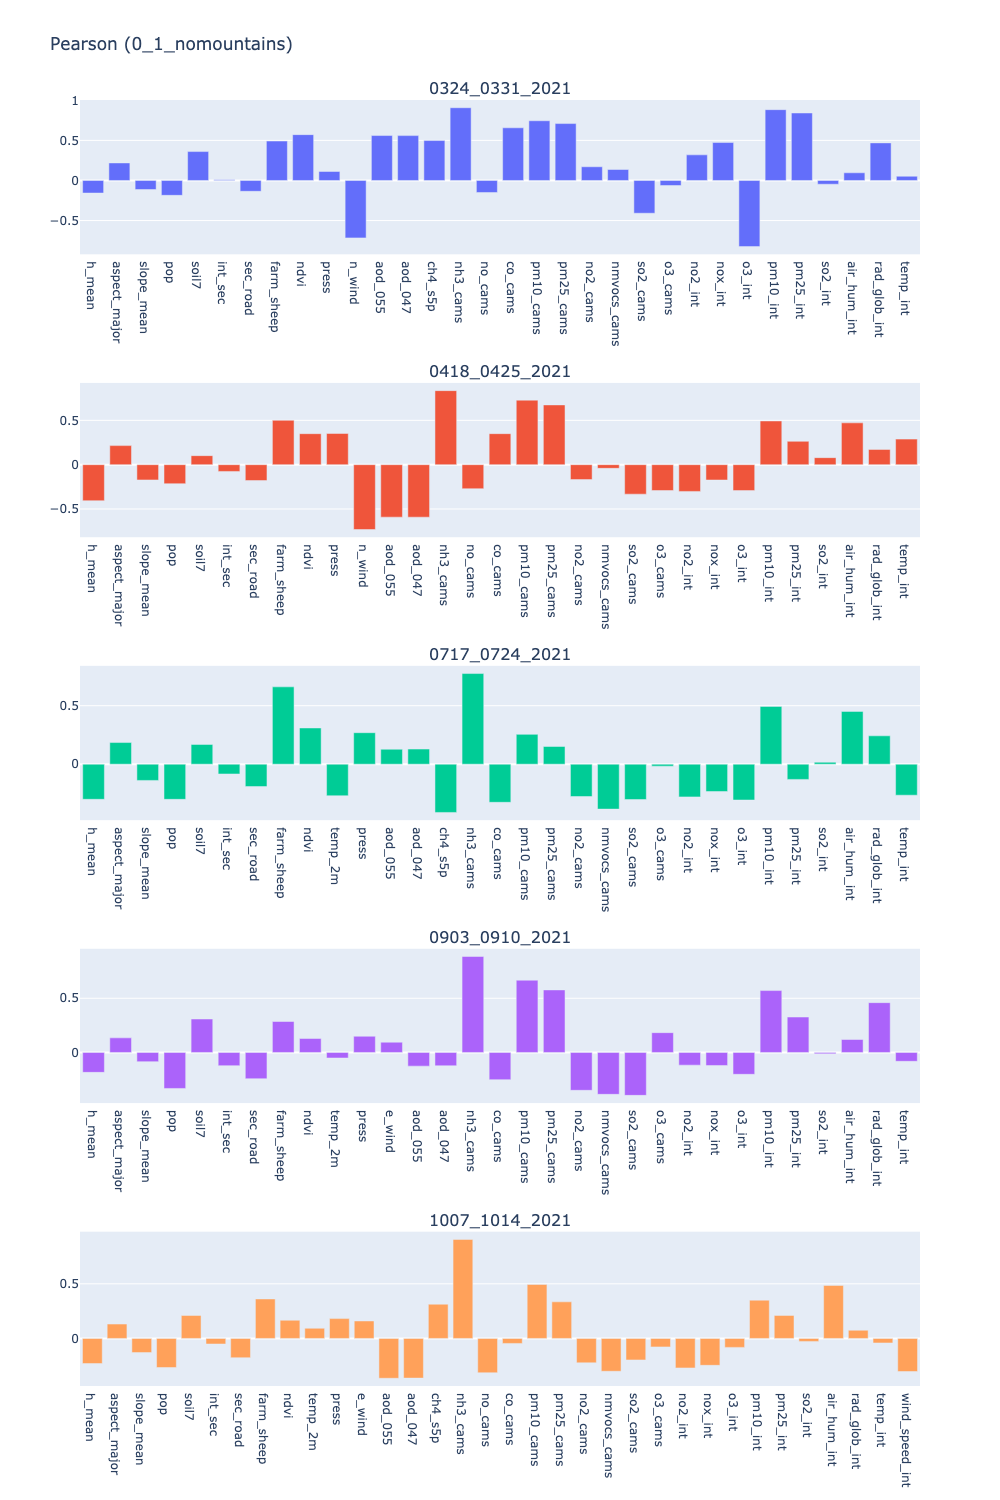
\includegraphics[scale=0.35]{images/tests/0_1_nomountainsnh3_st_pearson.png}
    \caption{Pearson correlation index results with respect to ammonia ('nh3\_st') as target variable, with 10km resolution excluding mountains.}
    \label{fig:overview}
\end{figure}
\begin{figure}[H]
    \centering
    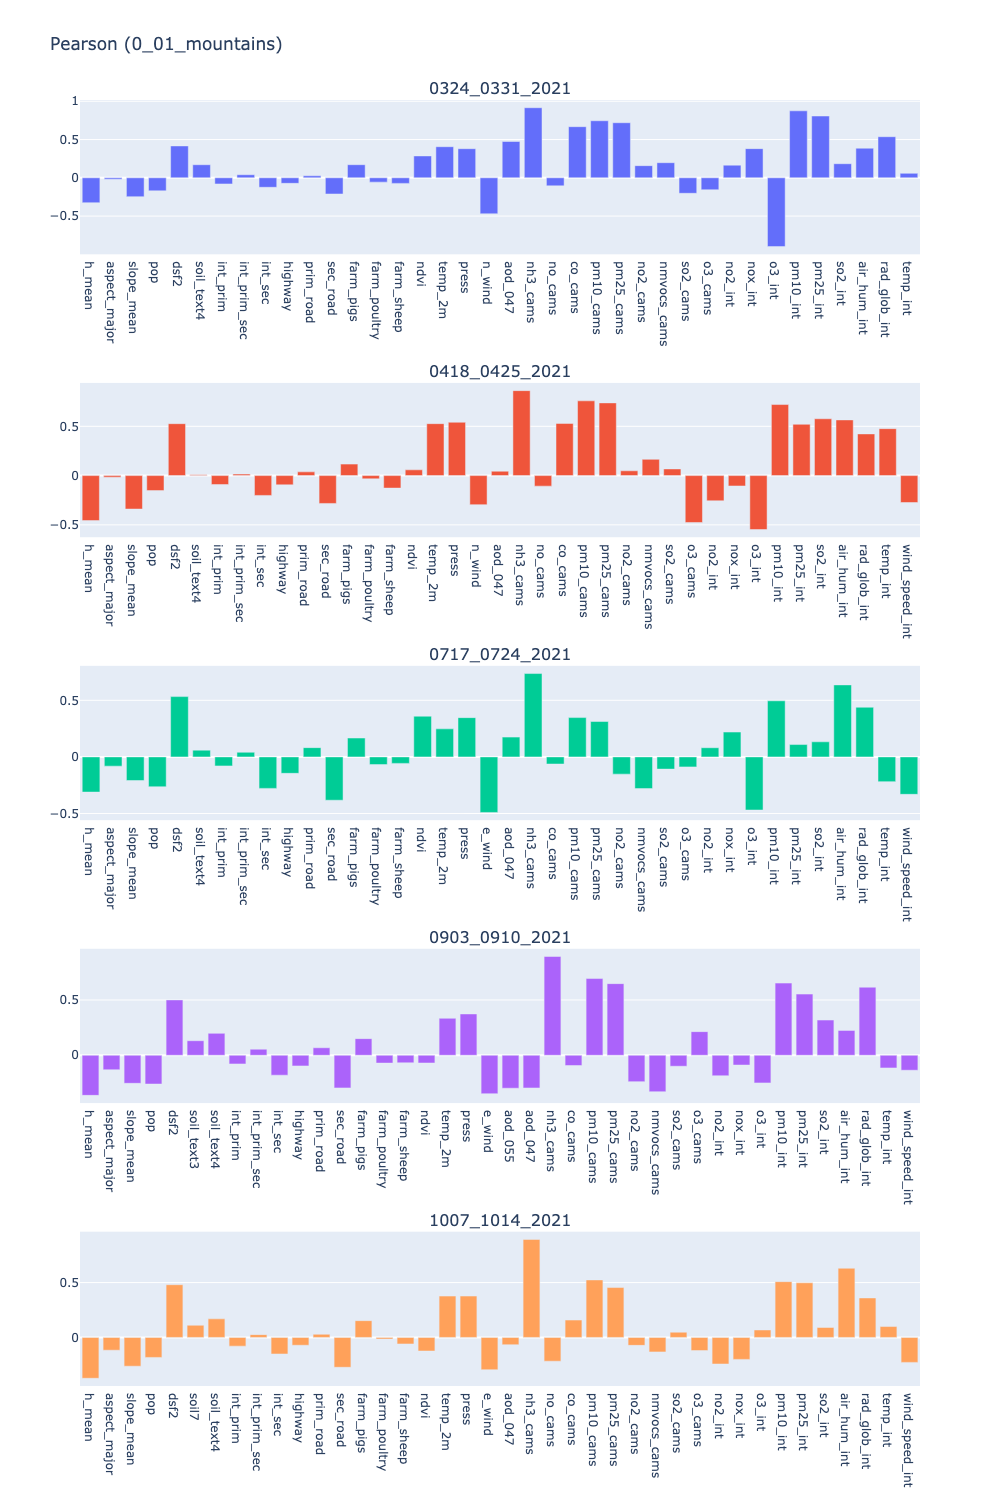
\includegraphics[scale=0.35]{images/tests/0_01_mountainsnh3_st_pearson.png}
    \caption{Pearson correlation index results with respect to ammonia ('nh3\_st') as target variable, with 1km resolution including mountains.}
    \label{fig:overview}
\end{figure}
\begin{figure}[H]
    \centering
    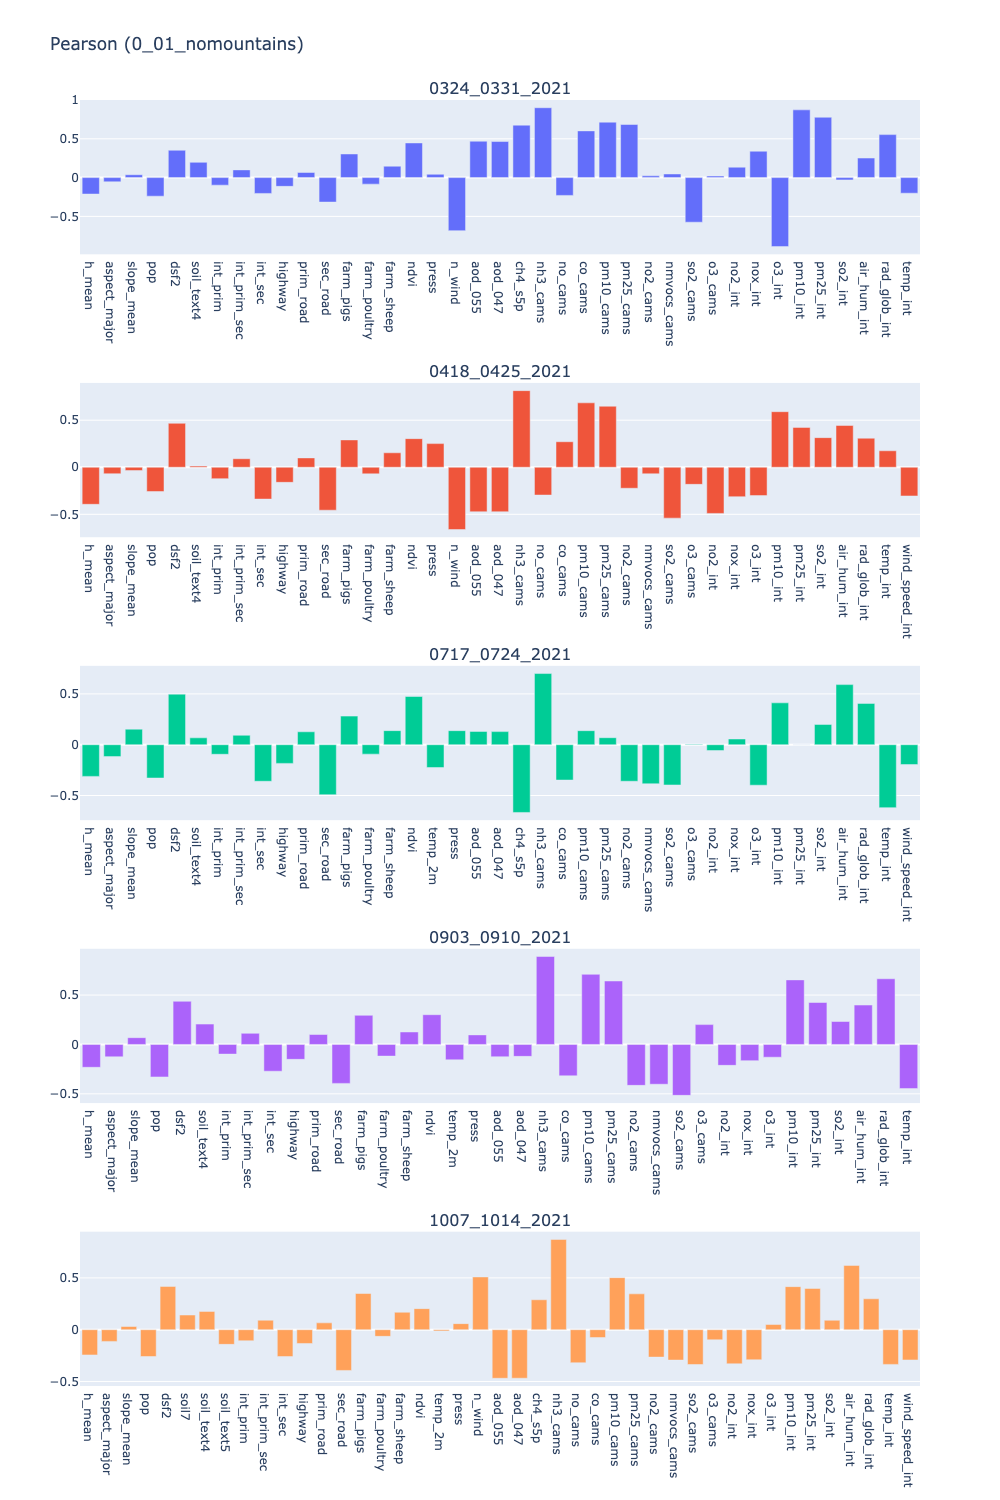
\includegraphics[scale=0.35]{images/tests/0_01_nomountainsnh3_st_pearson.png}
    \caption{Pearson correlation index results with respect to ammonia ('nh3\_st') as target variable, with 1km resolution excluding mountains.}
    \label{fig:overview}
\end{figure}

\section{ML models results}
\subsection{Random Forest}

\begin{table}[H]
\begin{tabular}{rrrrrr}
\hline
       &   24/03-31/03 &   18/04-25/04 &   17/07-24/07 &   3/09-10/09 &   7/10-14/10 \\
\hline
   MAE\_sensor   &1.777 &1.034 &0.796 &1.026 &0.893 \\
   MSE\_sensor   &7.483 &            1.967 &            1.035 &            2.018 &            1.287 \\
   R2\_sensor    & 0.709 &            0.714 &            0.494 &            0.813 &            0.839 \\
   MAE\_cams     &7.8   &            6.556 &            2.11  &            3.06  &3.478 \\
   MSE\_cams     &86.279 &           57.593 &            7.548 &           13.266 &16.591 \\
   R2\_cams&-2.147 &           -7.492 &           -2.846 &           -0.258 &           -1.096 \\
\hline
\end{tabular}
\caption{Random Forest prediction for PM2.5 with 10 km resolution, including zones with mountains.}
\end{table}
\bigskip
\begin{table}[H]
\begin{tabular}{rrrrrr}
\hline
      &   24/03-31/03 &   18/04-25/04 &   17/07-24/07 &   3/09-10/09 &   7/10-14/10 \\
\hline
  MAE\_sensor   &            2.114 &            1.329 &            0.825 &            1.311 &            0.752 \\
  MSE\_sensor   &            8.825 &            3.047 &            1.19  &            3.016 &            0.917 \\
  R2\_sensor    &            0.712 &            0.61  &            0.504 &            0.716 &            0.846 \\
  MAE\_cams     &            8.23  &            7.914 &            1.386 &            3.581 &            3.744 \\
   MSE\_cams     &           95.109 &           76.441 &            2.867 &           16.923 &           18.964 \\
   R2\_cams      &           -2.312 &           -8.546 &           -0.185 &           -0.632 &           -2.373 \\
\hline
\end{tabular}
\caption{Random Forest prediction for PM2.5 with 10 km resolution, excluding zones with mountains.}
\end{table}

\begin{table}[H]
\begin{tabular}{rrrrrr}
\hline
     &   24/03-31/03 &   18/04-25/04 &   17/07-24/07 &   3/09-10/09 &   7/10-14/10 \\
\hline
   MAE\_sensor   &            0.465 &            0.36  &            0.33  &            0.325 &            0.269 \\
  MSE\_sensor   &            0.654 &            0.333 &            0.266 &            0.291 &            0.174 \\
   R2\_sensor    &            0.983 &            0.962 &            0.926 &            0.98  &            0.979 \\
   MAE\_cams     &            8.966 &            7.566 &            1.936 &            3.574 &            3.974 \\
  MSE\_cams     &          106.414 &           71.818 &            6.213 &           16.81  &           20.988 \\
   R2\_cams      &           -1.821 &           -7.099 &           -0.727 &           -0.18  &           -1.578 \\
\hline
\end{tabular}
\caption{Random Forest prediction for PM2.5 with 1 km resolution, including zones with mountains.}
\end{table}


\begin{table}[H]
\begin{tabular}{rrrrrr}
\hline
      &   24/03-31/03 &   18/04-25/04 &   17/07-24/07 &   3/09-10/09 &   7/10-14/10 \\
\hline
  MAE\_sensor   &            0.586 &            0.445 &            0.344 &            0.365 &            0.362 \\
   MSE\_sensor   &            0.88  &            0.471 &            0.271 &            0.303 &            0.323 \\
  R2\_sensor    &            0.979 &            0.956 &            0.929 &            0.981 &            0.948 \\
  MAE\_cams     &            9.153 &            8.58  &            1.617 &            3.83  &            4.192 \\
   MSE\_cams     &          111.721 &           86.53  &            3.766 &           19.284 &           22.676 \\
  R2\_cams      &           -1.682 &           -7.131 &            0.004 &           -0.187 &           -2.674 \\
\hline
\end{tabular}
\caption{Random Forest prediction for PM2.5 with 1 km resolution, excluding zones with mountains.}
\end{table}

\begin{table}[H]
\begin{tabular}{rrrrrr}
\hline
      &   24/03-31/03 &   18/04-25/04 &   17/07-24/07 &   3/09-10/09 &   7/10-14/10 \\
\hline
   MAE\_sensor   &            4.864 &            1.359 &            4.016 &            4.907 &            1.967 \\
   MSE\_sensor   &           50.261 &            3.538 &           40.443 &           53.878 &           11.269 \\
  R2\_sensor    &            0.813 &            0.92  &            0.741 &            0.743 &            0.686 \\
   MAE\_cams     &           14.956 &           10.748 &            8.166 &           10.326 &            9.163 \\
  MSE\_cams     &          272.549 &          135.617 &          149.976 &          194.43  &          102.945 \\
   R2\_cams      &           -0.462 &           -2.048 &            0.013 &            0.139 &           -1.066 \\
\hline
\end{tabular}
\caption{Random Forest prediction for NH3 with 10 km resolution, including zones with mountains.}
\end{table}

\begin{table}[H]
\begin{tabular}{rrrrrr}
\hline
      &   24/03-31/03 &   18/04-25/04 &   17/07-24/07 &   3/09-10/09 &   7/10-14/10 \\
\hline
   MAE\_sensor   &            4.681 &            1.484 &            4.85  &            5.125 &            1.958 \\
   MSE\_sensor   &           48.004 &            5.385 &           54.68  &           53.327 &           12.165 \\
   R2\_sensor    &            0.823 &            0.868 &            0.464 &            0.642 &            0.845 \\
   MAE\_cams     &           15.383 &           10.758 &            8.942 &           10.304 &            9.497 \\
   MSE\_cams     &          288.521 &          138.082 &          178.69  &          211.569 &          110.82  \\
   R2\_cams      &           -0.022 &           -2.954 &           -0.236 &            0.062 &           -0.547 \\
\hline
\end{tabular}
\caption{Random Forest prediction for NH3 with 10 km resolution, excluding zones with mountains.}
\end{table}

\begin{table}[H]
\begin{tabular}{rrrrrr}
\hline
     &   24/03-31/03 &   18/04-25/04 &   17/07-24/07 &   3/09-10/09 &   7/10-14/10 \\
\hline
  MAE\_sensor   &            1.041 &            0.219 &            2.234 &            1.657 &            1.115 \\
  MSE\_sensor   &            6.883 &            0.149 &           23.044 &           15.641 &           14.283 \\
  R2\_sensor    &            0.985 &            0.998 &            0.911 &            0.964 &            0.933 \\
  MAE\_cams     &           17.694 &           10.536 &           11.049 &           13.329 &           11.48  \\
  MSE\_cams     &          343.112 &          145.433 &          287.761 &          382.879 &          169.03  \\
  R2\_cams      &            0.227 &           -1.134 &           -0.044 &            0.124 &           -0.03  \\
\hline
\end{tabular}
\caption{Random Forest prediction for NH3 with 1 km resolution, including zones with mountains.}
\end{table}


\begin{table}[H]
\begin{tabular}{rrrrrr}
\hline
     &   24/03-31/03 &   18/04-25/04 &   17/07-24/07 &   3/09-10/09 &   7/10-14/10 \\
\hline
  MAE\_sensor   &            1.293 &            0.238 &            2.25  &            2.304 &            1.504 \\
  MSE\_sensor   &           11.206 &            0.149 &           20.907 &           24.379 &           16.739 \\
  R2\_sensor    &            0.972 &            0.997 &            0.927 &            0.943 &            0.917 \\
  MAE\_cams     &           18.401 &           10.414 &           11.746 &           14.18  &           12.012 \\
  MSE\_cams     &          368.858 &          147.652 &          323.418 &          456.145 &          188.65  \\
  R2\_cams      &            0.136 &           -1.511 &           -0.158 &           -0.001 &           -0.06  \\
\hline
\end{tabular}
\caption{Random Forest prediction for NH3 with 1 km resolution, excluding zones with mountains.}
\end{table}


\subsection{Neural Network by Keras}

\begin{table}[H]
\begin{tabular}{rrrrrr}
\hline
     &   24/03-31/03 &   18/04-25/04 &   17/07-24/07 &   3/09-10/09 &   7/10-14/10 \\
\hline
  MAE\_sensor   &            2.095 &            1.591 &            0.867 &            1.61  &            1.193 \\
  MSE\_sensor   &            6.555 &            4.351 &            1.275 &            4.603 &            2.416 \\
  R2\_sensor    &            0.763 &            0.313 &            0.329 &            0.572 &            0.687 \\
  MAE\_cams     &            7.8   &            6.554 &            2.113 &            3.06  &            3.478 \\
  MSE\_cams     &           86.279 &           57.562 &            7.565 &           13.266 &           16.591 \\
  R2\_cams      &           -2.147 &           -8.102 &           -3.386 &           -0.239 &           -1.158 \\
\hline
\end{tabular}
\caption{Neural Network prediction for PM2.5 with 10 km resolution, including zones with mountains.}
\end{table}

\begin{table}[H]
\begin{tabular}{rrrrrr}
\hline
    &   24/03-31/03 &   18/04-25/04 &   17/07-24/07 &   3/09-10/09 &   7/10-14/10 \\
\hline
  MAE\_sensor   &            2.242 &            1.673 &            0.957 &            1.545 &            1.23  \\
 MSE\_sensor   &            7.436 &            4.204 &            1.622 &            4.119 &            2.558 \\
  R2\_sensor    &            0.737 &            0.505 &            0.315 &            0.634 &            0.557 \\
  MAE\_cams     &            8.243 &            7.907 &            1.383 &            3.581 &            3.744 \\
  MSE\_cams     &           95.313 &           76.364 &            2.859 &           16.923 &           18.964 \\
  R2\_cams      &           -2.281 &           -8.213 &           -0.193 &           -0.561 &           -2.351 \\
\hline
\end{tabular}
\caption{Neural Network prediction for PM2.5 with 10 km resolution, excluding zones with mountains.}
\end{table}

\begin{table}[H]
\begin{tabular}{rrrrrr}
\hline
    &   24/03-31/03 &   18/04-25/04 &   17/07-24/07 &   3/09-10/09 &   7/10-14/10 \\
\hline
  MAE\_sensor   &            1.609 &            1.157 &            0.783 &            1.247 &            0.776 \\
 MSE\_sensor   &            5     &            2.638 &            1.128 &            2.354 &            1.121 \\
  R2\_sensor    &            0.866 &            0.709 &            0.685 &            0.835 &            0.861 \\
  MAE\_cams     &            8.966 &            7.567 &            1.936 &            3.574 &            3.974 \\
  MSE\_cams     &          106.423 &           71.82  &            6.214 &           16.811 &           20.987 \\
  R2\_cams      &           -1.84  &           -6.979 &           -0.735 &           -0.157 &           -1.585 \\
\hline
\end{tabular}
\caption{Neural Network prediction for PM2.5 with 1 km resolution, including zones with mountains.}
\end{table}


\begin{table}[H]
\begin{tabular}{rrrrrr}
\hline
    &   24/03-31/03 &   18/04-25/04 &   17/07-24/07 &   3/09-10/09 &   7/10-14/10 \\
\hline
  MAE\_sensor   &            1.584 &            0.829 &            0.583 &            0.752 &            0.523 \\
  MSE\_sensor   &            3.932 &            1.229 &            0.646 &            0.906 &            0.559 \\
  R2\_sensor    &            0.906 &            0.883 &            0.826 &            0.945 &            0.911 \\
  MAE\_cams     &            9.153 &            8.581 &            1.617 &            3.83  &            4.192 \\
  MSE\_cams     &          111.72  &           86.539 &            3.766 &           19.282 &           22.673 \\
  R2\_cams      &           -1.627 &           -7.082 &           -0.006 &           -0.181 &           -2.616 \\
\hline
\end{tabular}
\caption{Neural Network prediction for PM2.5 with 1 km resolution, excluding zones with mountains.}
\end{table}


\begin{table}[H]
\begin{tabular}{rrrrrr}
\hline
    &   24/03-31/03 &   18/04-25/04 &   17/07-24/07 &   3/09-10/09 &   7/10-14/10 \\
\hline
  MAE\_sensor   &            6.248 &            3.253 &            5.565 &            7.325 &            4.305 \\
  MSE\_sensor   &           71.133 &           19.21  &           74.444 &          123.832 &           51.589 \\
  R2\_sensor    &            0.708 &            0.479 &            0.505 &            0.511 &            0.372 \\
  MAE\_cams     &            6.66  &            4.05  &            7.537 &            6.583 &            2.601 \\
 MSE\_cams     &           69.718 &           31.198 &          115.937 &          102.716 &           13.809 \\
  R2\_cams      &            0.68  &            0.217 &            0.212 &            0.546 &            0.822 \\
\hline
\end{tabular}
\caption{Neural Network prediction for NH3 with 10 km resolution, including zones with mountains.}
\end{table}

\begin{table}[H]
\begin{tabular}{rrrrrr}
\hline
    &   24/03-31/03 &   18/04-25/04 &   17/07-24/07 &   3/09-10/09 &   7/10-14/10 \\
\hline
   MAE\_sensor   &            6.147 &            2.593 &            5.095 &            6.807 &            3.315 \\
  MSE\_sensor   &           72.241 &           12.389 &           45.941 &           82.49  &           26.293 \\
  R2\_sensor    &            0.737 &            0.62  &            0.6   &            0.547 &            0.666 \\
  MAE\_cams     &            7.283 &            4.559 &            8.412 &            7.581 &            3.033 \\
  MSE\_cams     &           78.979 &           36.499 &          135.704 &          123.934 &           16.818 \\
  R2\_cams      &            0.71  &           -0.106 &           -0.034 &            0.425 &            0.591 \\
\hline
\end{tabular}
\caption{Neural Network prediction for NH3 with 10 km resolution, excluding zones with mountains.}
\end{table}

\begin{table}[H]
\begin{tabular}{rrrrrr}
\hline
    &   24/03-31/03 &   18/04-25/04 &   17/07-24/07 &   3/09-10/09 &   7/10-14/10 \\
\hline
  MAE\_sensor   &            3.27  &            1.893 &            2.558 &            2.866 &            1.79  \\
  MSE\_sensor   &           30.434 &            9.657 &           12.184 &           14.442 &            5.497 \\
  R2\_sensor    &            0.933 &            0.864 &            0.952 &            0.967 &            0.966 \\
  MAE\_cams     &            8.197 &            4.031 &           10.073 &            9.247 &            4.327 \\
  MSE\_cams     &          118.847 &           38.357 &          225.879 &          243.268 &           51.953 \\
  R2\_cams      &            0.736 &            0.456 &            0.18  &            0.445 &            0.695 \\
\hline
\end{tabular}
\caption{Neural Network prediction for NH3 with 1 km resolution, including zones with mountains.}
\end{table}


\begin{table}[H]
\begin{tabular}{rrrrrr}
\hline
    &   24/03-31/03 &   18/04-25/04 &   17/07-24/07 &   3/09-10/09 &   7/10-14/10 \\
\hline
  MAE\_sensor   &            2.372 &            1.378 &            3.905 &            3.307 &            1.974 \\
  MSE\_sensor   &           10.518 &            3.907 &           24.668 &           25.564 &            6.533 \\
  R2\_sensor    &            0.975 &            0.937 &            0.906 &            0.948 &            0.947 \\
  MAE\_cams     &            9.253 &            4.56  &           11.334 &           11.259 &            5.461 \\
  MSE\_cams     &          135.675 &           43.816 &          257.91  &          306.085 &           67.695 \\
  R2\_cams      &            0.692 &            0.254 &            0.058 &            0.342 &            0.631 \\
\hline
\end{tabular}
\caption{Neural Network prediction for NH3 with 1 km resolution, excluding zones with mountains.}
\end{table}









